\documentclass[11pt]{article}

\usepackage{fullpage}
\usepackage{url}
\usepackage{paralist}
\usepackage[pdftex]{graphicx}
\usepackage{epstopdf}
\usepackage[small]{caption}
\usepackage{subfig}
\usepackage{multirow}

% =========
\usepackage{color}

% The xxx tag is intended to denote urgent text that needs addressing.
% The meh tag is intended to highlight text that needs some loving or which
% we're not sure should make primetime
\newcommand{\xxx}[1]{{\bf \color{red} #1}}
\newcommand{\meh}[1]{{\bf \color{blue} #1}}
\newcommand\T{\rule{0pt}{3ex}}
\newcommand\B{\rule[-1.2ex]{0pt}{0pt}}

% =========

\title{Learning a Visual Vocabulary: Identifying Objects
    Through Learned Verbal Commands}
\author{Rob Goeddel \and Lauren Hinkle \and James Kirk \and Aaron Mininger}
\date{}

\begin{document}
\maketitle

\begin{abstract}
Interaction between robots and humans is a rapidly growing area of reasearch. Of particular interest is the desire to interact with robots or agents using natural language. This gives humans a more natural and effective way of teaching, commanding, and interacting with robotic agents or computers. Our work is designed to process images and provide descriptions of objects that can then be used in interactions with humans. We use images from a RGB-D camera in order to classify properties of objects including size, shape, and color. Those descriptions are then fed into a higher-level agent which handles the human interaction. We specifically use a simple I-Spy game to allow users to refer to objects using descriptions in natural language.
\end{abstract}

\section{Introduction}
%\xxx{Problem description and motivation. Why do you want to solve this
%    problem? What's the impact if you can solve this problem?}
Language is a powerful tool that is just coming into its own as the human
interface for various systems. Apple's Siri is an excellent example of this, making interaction with your phone intuitive, easy, and efficient. Robotic systems in AI can also benefit from greater understanding of
language. Such knowledge could allow a human to command or teach a robot agent in a more natural way. Take, for example, a robotic arm system with knowledge of only
several nouns and actions: cup, sink, grab/move object, and turning on/off
the sink, and the spatial concept of in. Through language, the robot could then be taught the new action of ``filling a cup'', which means to put the cup in the sink and turn on the
sink. Even though the robot has never seen anyone fill a cup before, now
it should be able to do so itself. Furthermore, the agent could generalize the concept to new items, like a bowl. This is a powerful
way for an agent to learn from a human, without requiring expert instructors.

Our goal is to leverage machine learning techniques in order to train a system to know a small vocabulary of nouns, adjectives,
and actions. As a proof of concept, we want to be able to play the children's
game ``I spy'' with a robotic arm. The arm's ``eyes'' will be a Microsoft
Kinect (or, with some small probability, a stereo camera rig) capable of
returning RGB-D data for classification. A collection of objects will be placed in the view of the camera, and a person will give a description of one of the objects. The agent will then select the object that matches that description using the robot arm.

This work is planned to be incorporated into a larger project which includes teaching the agent new concepts and actions as described above. Such a project relies on having symbolic information provided by our work through object segmentation and classification. The low level features provided by our system can be analyzed and combined in order to build new concepts like object categories (like blocks and balls) or object properties (all bananas are yellow). Such reasoning and concept generalization is essential for agents that interact in novel situations. These capabilities could be used on service tasks or with non-robotic systems where a verbal interface
offers improvements in efficiency, safety, etc.

\section{Proposed Method}
%\xxx{How are you going to solve this problem? Why should the proposed method
%    work? Provide technical details of your approach if you are proposing a
%    novel method.}

Our approach will use supervised learning techniques to generate a description of each object. First, we will gather our training data by collecting a number of RGB-D images from the camera featuring various types and positions of objects. Each image will be run through a segmentation process to isolate every object in the scene. Each object will be manually given a label describing its color, shape, and size. From these segmentations we will extract a useful feature vector for each attribute. One of the main challenges for good object classification will be designing a
diverse and robust feature space to recognize the object characteristics we
are interested in. Color presents easy features such as RGB and HSV
descriptions. Volume computations and bounding box dimensions based on
relations to the other objects in the scene can give us scale information
necessary for estimating relative size. Shape is a more complex matter,
especially given the noise seen in the Kinect data. We plan on exploring
spherical harmonics, edge/corner features, and features based on projected
models of missing data (for example, symmetry) to correctly identify shapes.
Once the features are extracted, we need to use a machine learning algorithm to perform the classification. We decided to use the liblinear SVM ~\cite{LIBLINEAR} because it is widely used, powerful, reliable, and performs well for classification tasks. We are specifically using multiclass approach because we have attributes like color which can take on several discrete values.

For object identification we will do a similar process to segment each object in the camera's image. That object's position in 3D space will be determined using both the pixel coordinate and the depth value. The features will then be extracted and run through our SVM's using the models created with the training data. This will give us a bag of words description for each object in the scene. This description, along with the position, will be given as input to a Soar agent. Soar is a cognitive architecture that will be responsible for the high-level reasoning and language processing. Our Soar agent will interpret the commands given by the users, determine which object is being described, and give the appropriate commands to the robotic arm.


\section{Related Work}
%\xxx{What are existing methods? What are the state-of-the-art methods for this
%    problem? How is your approach different from the related work?}
Object classification is a problem that appears throughout a variety of applications, ranging from law enforcement to manufacturing. While historic efforts have focused more on the recognition problem, that is, finding a known object in a scene, more recent work has emphasized the more general problem of classifying objects into generic groups by type [Huber]. For example, we might be interested in identifying vehicles as bikes, motorcycles, trucks, cars, etc. Work by [Nilsback] and [Gehler], among others, has shown that powerful classifiers may be constructed through boosting or similar across simple feature-specific classifiers such as color, shape, etc.

Recent popularization of sensors that combine both image and depth information like the Microsoft Kinect inexpensively provide richer sensory information. The addition of depth can help disambiguate situations that would be very difficult with a normal camera image alone. Depth can make the determination of an object’s underlying geometry much easier, leading to better identification [Marton]. Previous work has successfully incorporated such cameras (often called RGBD cameras) with object recognition in indoors domains featuring common household objects [Marton, Lai].

Our work will approach this problem from a different direction. Instead of learning how to combine different feature spaces to describe different classes of objects, we will learn words that describe regions of our feature spaces that may then be combined to describe classes of objects. For example, trash cans in CSE may be described as blue or gray rectangular prisms. This allows us to quickly come up with classifiers for new object classes since we may construct them from our learned vocabulary instead of learning models of them directly in feature space.


\section{Experimental Results}
\subsection{Infrastructure}
We have begun building several of the pieces necessary for our I-spy
game in parallel.  Prof. Edwin Olson has supplied the group with a robotic
arm (pictured in Figure~\ref{fig:arm}) and a Kinect.  We built an
overhead mount (pictured in Figure~\ref{fig:kinect-mount}) to allow the Kinect
to view a small (~2\,ft $\times$ 4\,ft) play area.

We calibrated the Kinect using an external package~\xxx{cite}, but may still
choose to calibrate it ourselves using several independent tools to see if we
can improve the calibration error. We are using the OpenKinect
package libfreenect~\cite{OpenKinect} to acquire data from the Kinect.  We have
written a small driver in C to output frames via LCM~\cite{huang2010} to simplify
communication with the driver for our Java code.  LCM also offers useful
built-in logging capabilities.

\begin{figure}
\centering
\subfloat[Robotic arm] {
    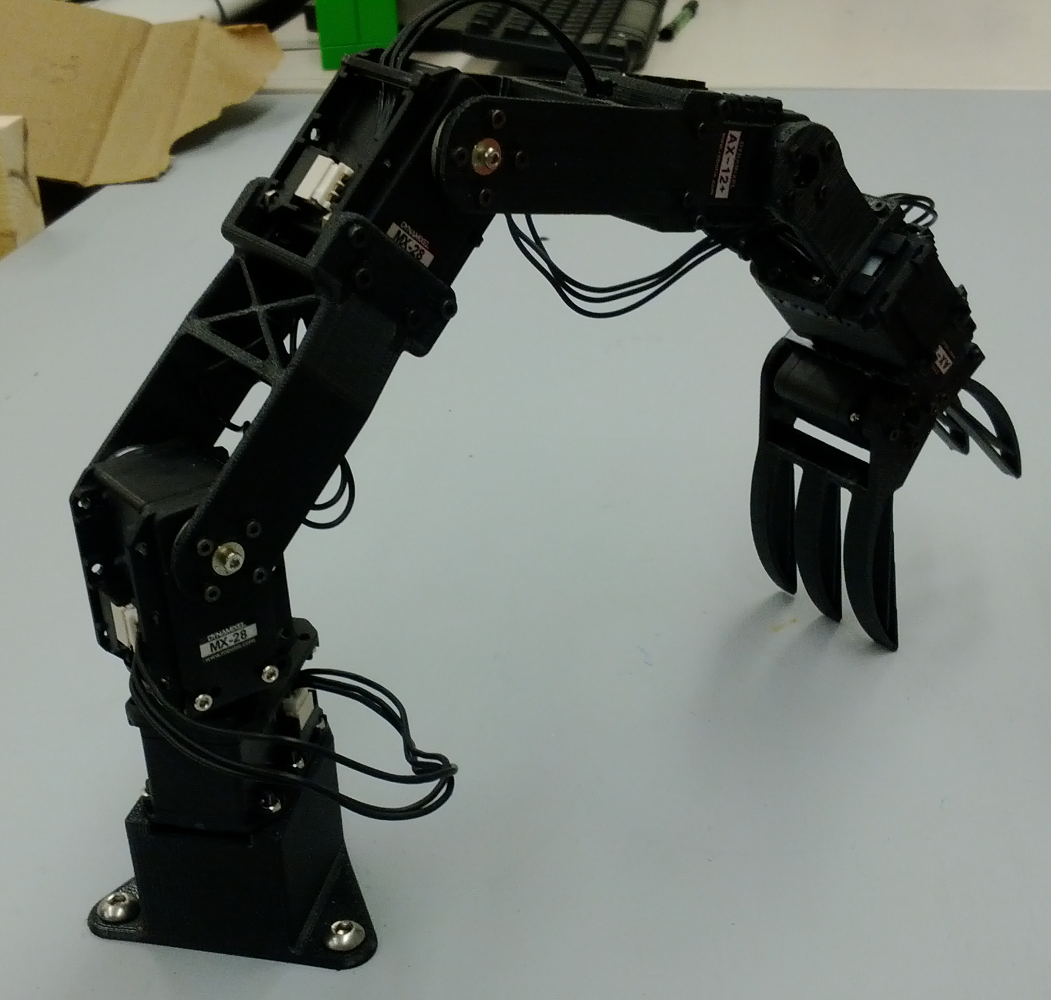
\includegraphics[height=2.5in]{figures/arm2.png}
    \label{fig:arm}
}
\subfloat[Kinect camera mount] {
    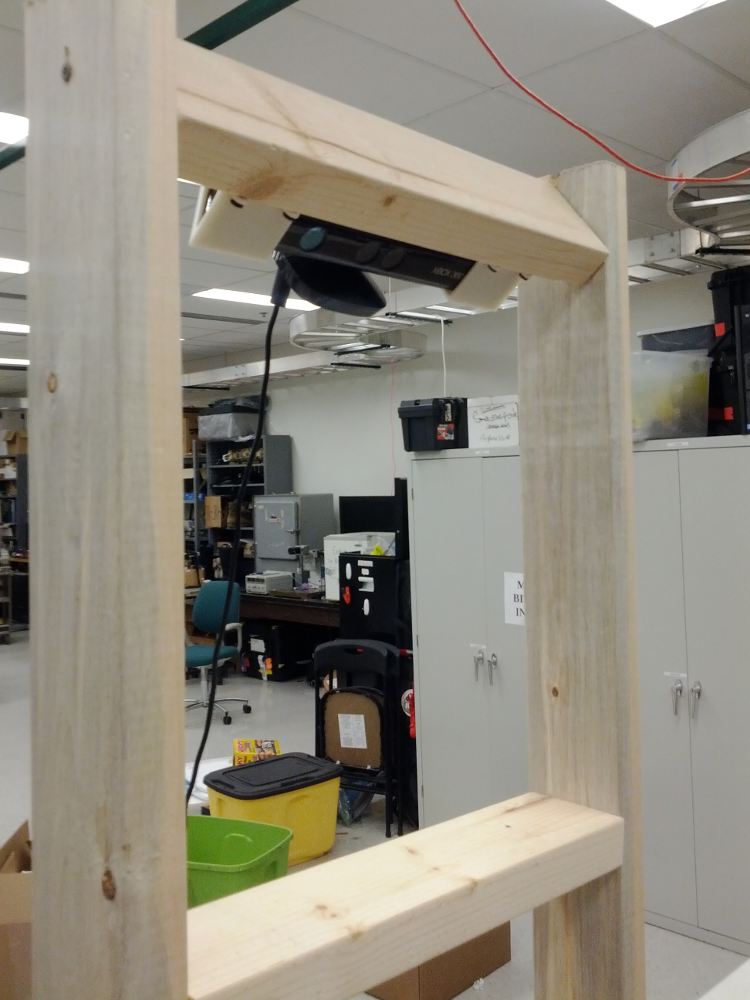
\includegraphics[height=2.5in]{figures/kinect.png}
    \label{fig:kinect-mount}
}
\caption{The hardware components used by our project that sense and interact with the environment.}
\label{fig:hardware}
\end{figure}

\subsection{Data Collection and Training}
We have acquired a large variety of children's foam blocks in many shapes, sizes,
and colors to act as our objects for classification. A small subset of the
blocks can be seen in Figure~\ref{fig:blocks}. The foam of the blocks is an
ideal material to work with as it
\begin{inparaenum}[(1)]
\item has a smooth, matte finish,
\item comes in a variety of distinct colors, and
\item is deformable enough to be grabbed by the arm but still retain its
shape.
\end{inparaenum}

We have collected a training dataset of footage of the foam blocks at numerous
positions and angles throughout the play area. We have created a tool that
segments out objects from the scene and allows a human to label these objects
with relevant descriptors.  We are still working on further developing this
tool to ease the process of labeling this large amount of data.


We have initially focused on getting some of the data labeled with colors so as
to do an SVM classification to validate our method.  With a small amount of
data labeled we have successful used the liblinear software~\cite{LIBLINEAR} to do
binary classification of colors.  The dimensions used for training were the
Red, Green, Blue, Saturation, Hue, and Value means for each object.  Binary
classifications between any two colors, even close colors like blue and purple,
were able to achieve near 100 percent accuracy.  Although this was just will a
small subset of data, this is still encouraging and helps somewhat ameliorate
the concerns that the Kinect system will produce clean enough data, at least in
the case of color.  More investigation and evaluation will occur once other
features, such as shape, are explored.

This is a multi-class classification problem so we intend to use a one-vs-all
(OVA) approach.  However with the only small amount of data that has been
labeled so far (pictured in Figure~\ref{fig:colordata}), the OVA
classification did not perform very well. The results in Table~\ref{tbl:testresults} show plenty of room for improvement. This should
be addressed once we have a more efficient system for labeling the data
collected.  If the OVA approach still proves problematic, we are also
considering using a strategy where a set of binary, one-vs-one, classifiers are
used.  The result is determined by which class is selected by most classifiers.

\pagebreak
\begin{figure}
\centering
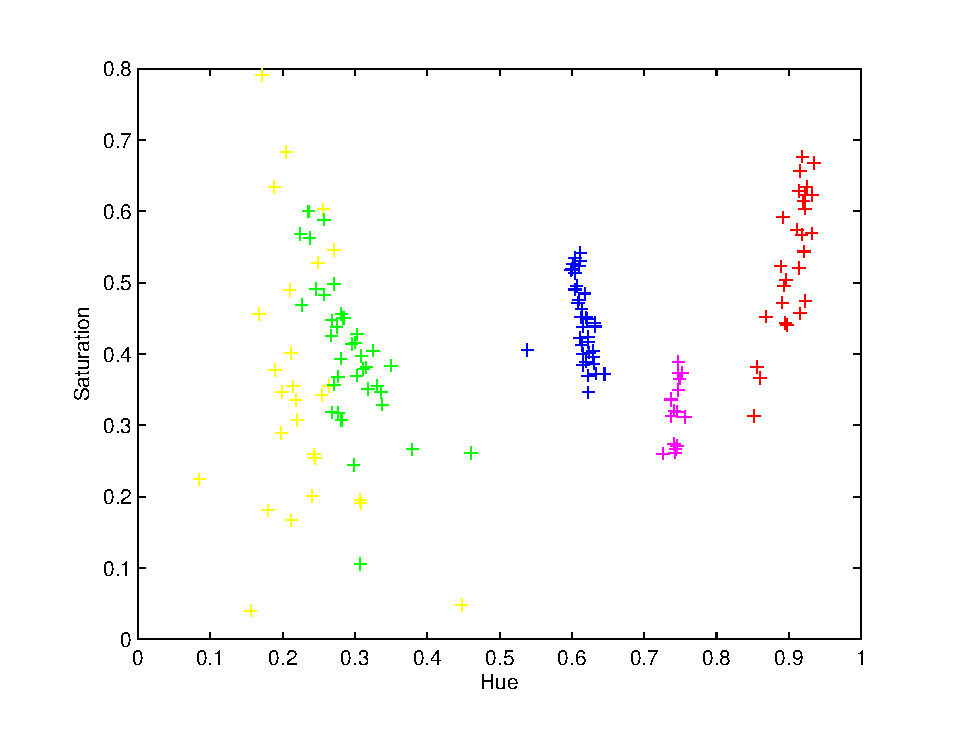
\includegraphics[height=1.75in]{figures/colorplot_noorange.eps}
\caption{Our distribution of real-world color data in hue and saturation
    dimensions. Point colors correspond with the ground truth color labeling,
    so true red examples are shown as red +s.}
\label{fig:colordata}
\end{figure}

\begin{figure}
\centering
\subfloat[Foam Blocks] {
    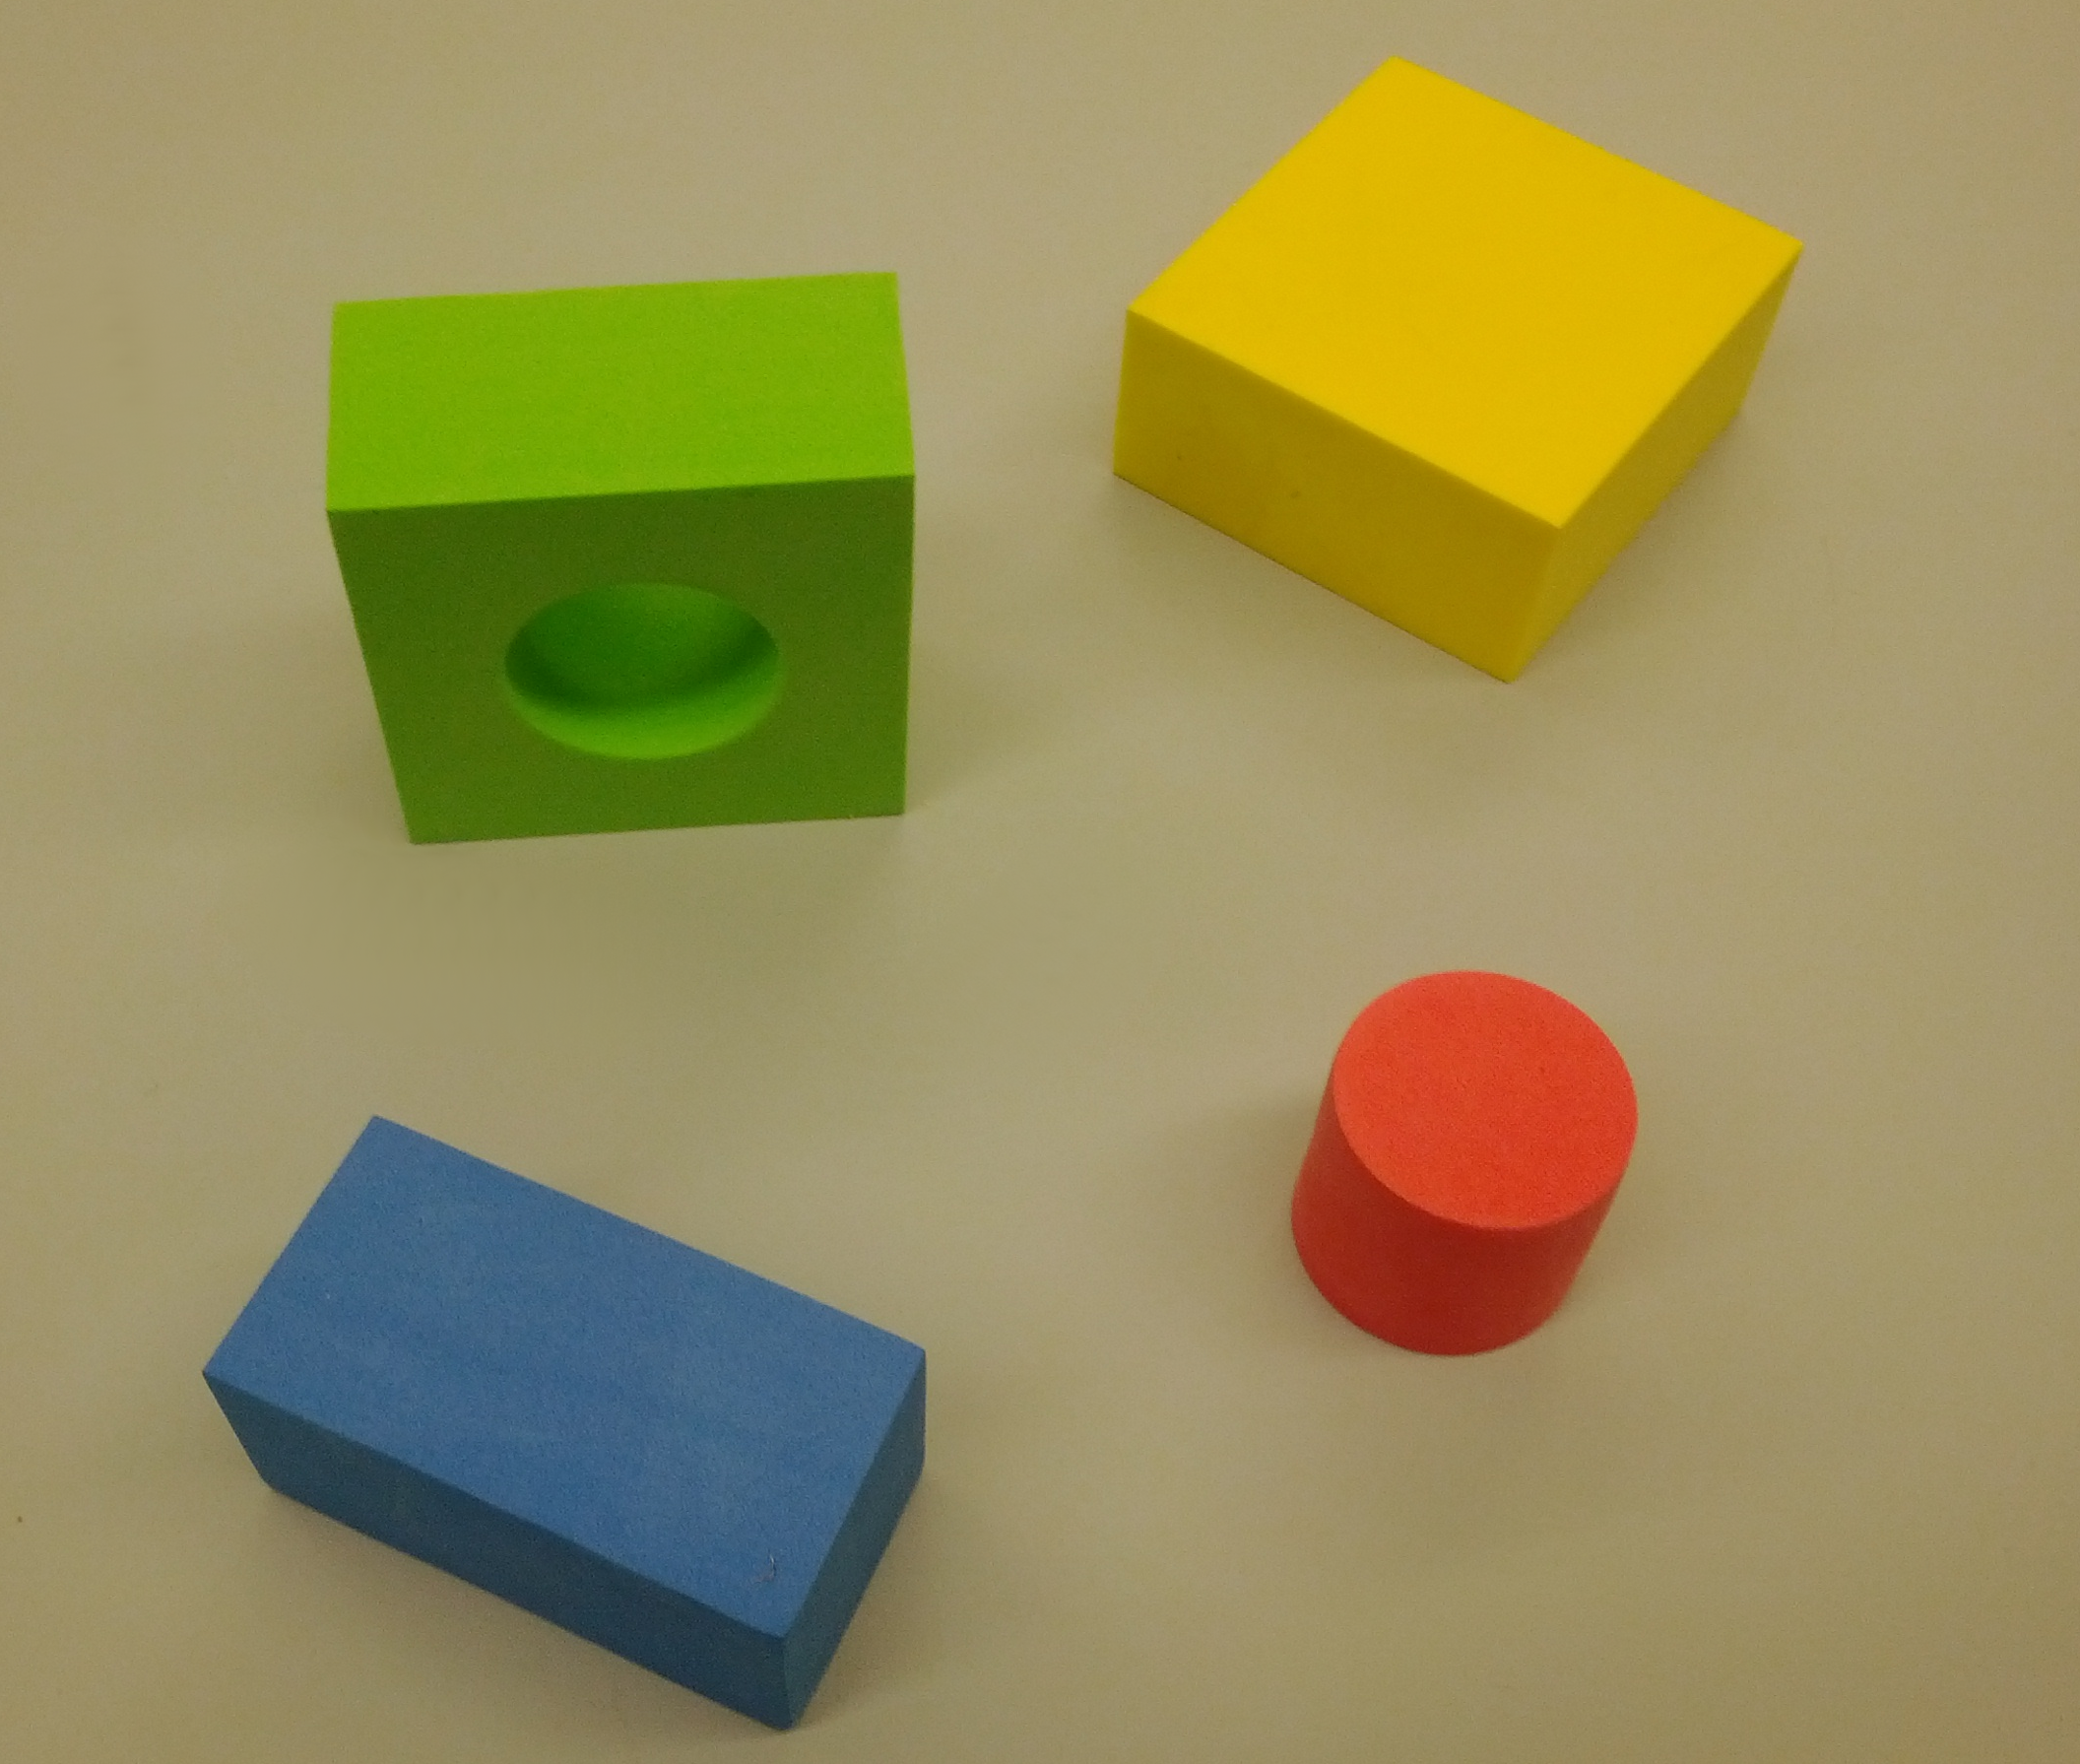
\includegraphics[height=1.75in]{figures/blocks.png}
    \label{fig:blocks}
}
\subfloat[Segmented Images] {
    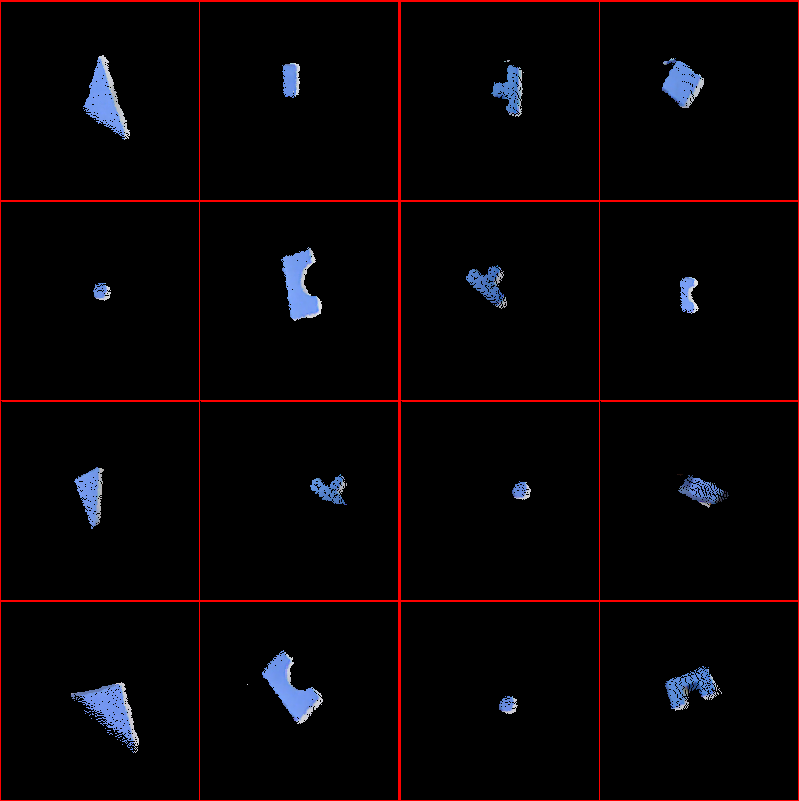
\includegraphics[height=1.75in]{figures/blue_objs.png}
    \label{fig:images}
}
\caption{On the left are the foam blocks used in our system. The objects are limited to simple shapes and colors. On the right is the segmented data from the camera which will be used for feature extraction}
\label{fig:objects}
\end{figure}

% orange 87.10
\begin{table}
\centering
\begin{tabular}{ | l | l | l | l | l | l |}
    \hline
    red &  yellow & green & blue & purple \T \B \\ \hline
    96.43\%  & 92.00\% & 97.37 \% & 100.00\% & 88.57\% \B \T \\ \hline
\end{tabular}
\caption{This shows the result of OVA classification for five color types
    across 160 objects. Each test involved training on 80\% of the points,
           with 20\% left out for testing.}
\label{tbl:testresults}
\end{table}
\pagebreak

\section{Future Milestones}
Our estimated schedule for the future can be seen in the table below. By early
April, we hope to have the plumbing completely done and at least color working
fully, giving us bare minimum successful performance. After this point, we
will focus on extending our feature space.

\begin{center}
    \begin{tabular}{ | l | l |}
    \hline
    \multirow{2}{*}{11~Mar -- 17~Mar}
	& Full labeling of the training data \T \\
	& SVM trained using the color features \B \\
    \hline
    \multirow{2}{*}{18~Mar -- 24~Mar}
	& Evaluation and tuning of color classification \T \\
	& Object Localization (determining an object's position in 3D space) \B \\
    \hline
    \multirow{2}{*}{25~Mar -- 31~Mar}
	& Focus our time on the Machine Learning midterm \T\\
	& Have all the components of our system connected together ('water through the pipes') \B \\
    \hline
    \multirow{2}{*}{1~Apr -- 7~Apr}
	& Test and debug the first assembled version of the system \T \\
	& Add shape/size features and classification to the system \B\\
    \hline
    \multirow{2}{*}{8~Apr -- 14~Apr}
	& Verify that we can distinguish two objects with different features \T\\
	& Evaluation and tuning of our shape/size classification \B \\
    \hline
    \multirow{3}{*}{15~Apr -- 21~Apr}
	& Implement the user interface, including the 'I Spy' game format \T\\
	& Full evaluation of the system \\
	& Start writing up the report and the poster \B \\
    \hline
    \multirow{3}{*}{21~Apr -- 24~Apr}
	& Finish editing final report \T \\
	& Finish editing poster and print final copy \\
	& Prepare and practice the presentation \B \\
    \hline
    \end{tabular}
\end{center}

\section{Conclusion}
%\xxx{Summary of your progress and your final expected goal (what do you expect
%    to achieve or demonstrate for the final project?)}
Our primary focus in the project has been setting up all the parts we need to move forward with the core of the project. This includes getting the camera and installing it in a rig, connecting to the camera to get the data, and acquiring the necessary training data. We are in the process of getting labeled feature representations out of that data in order to train an SVM on it. Our preliminary tests using color data indicate that our color classification method will be sufficient to distinguish between colors with high accuracy.

In the end, we want our system to provide a discription for each object that is accurate and robust. This will ensure that our agent is able to correctly identifiy the objects described within the context of our I Spy game. We expect that shape will be more prone to noise and error than color, but we would still like our agent to correctly identify the shape at least 90\% of the time. Misclassification errors made by the visual system can have very detrimental effects on the high-level system using those classifications, so our top priority is to provide object descriptions that are as noiseless and error-free as possible.

\bibliographystyle{plain}
\bibliography{literature}

\end{document}
